%%%
% Conférence « Comment bien démarrer son projet »
% Vendredi 03 décembre 2010
%%%

\section{Subversion}

\subsection{Généralités}
\begin{frame}{Pourquoi versionner~?}
  \begin{alertblock}{Concrètement}
    SVN vous permet de~:
    \begin{itemize}
      \item gérer votre code source,
      \item conserver une trace toutes les modifications,

      \item revenir en arrière,
      \item travailler à plusieurs en partageant le code intelligement.
    \end{itemize}
  \end{alertblock}
  \begin{center}
    
\includegraphics[scale=3]{images/logo_svn}
  \end{center}
\end{frame}

\subsection{Utilisation typique}

\begin{frame}
  \begin{center}
    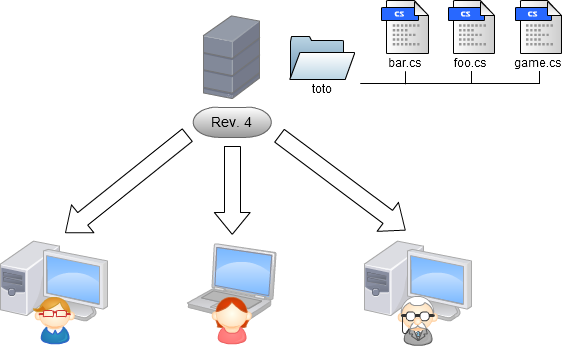
\includegraphics[scale=0.52]{images/1-CheckOut.png}
  \end{center}
\end{frame}

\begin{frame}
  \begin{center}
    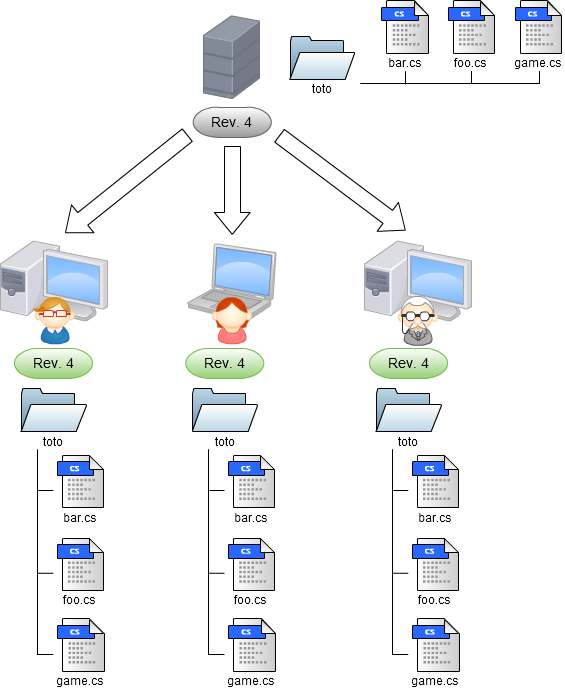
\includegraphics[scale=0.3]{images/2-CheckOut.png}
  \end{center}
\end{frame}

\begin{frame}
  \begin{center}
    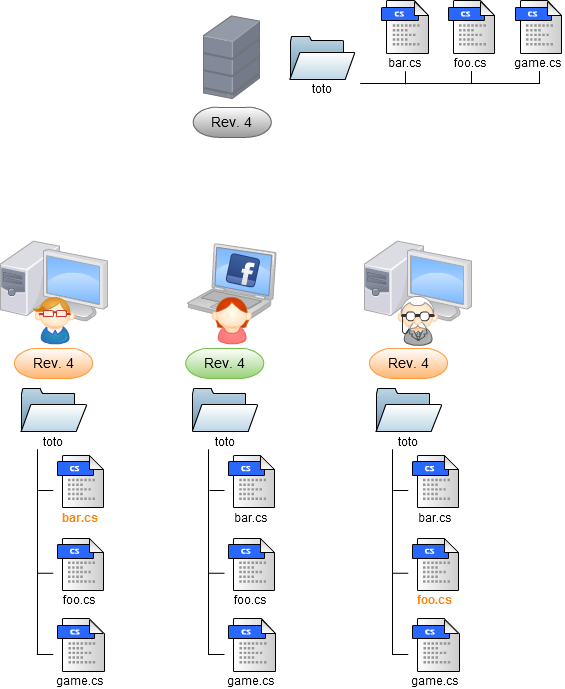
\includegraphics[scale=0.3]{images/3-Work.png}
  \end{center}
\end{frame}

\begin{frame}
  \begin{center}
    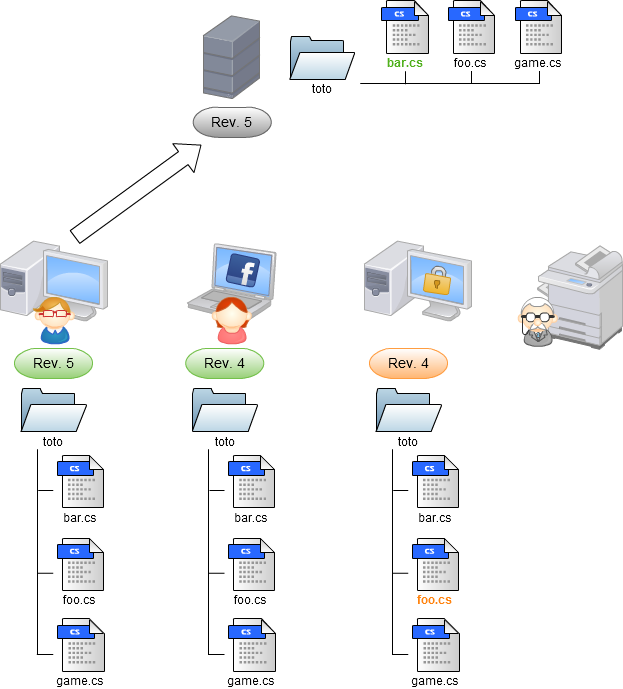
\includegraphics[scale=0.3]{images/4-Commit1.png}
  \end{center}
\end{frame}

\begin{frame}
  \begin{center}
    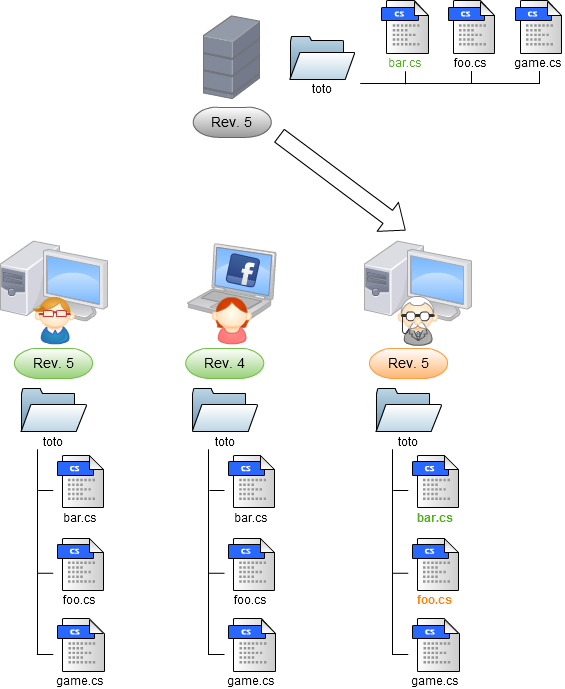
\includegraphics[scale=0.3]{images/5-Update.png}
  \end{center}
\end{frame}

\begin{frame}
  \begin{center}
    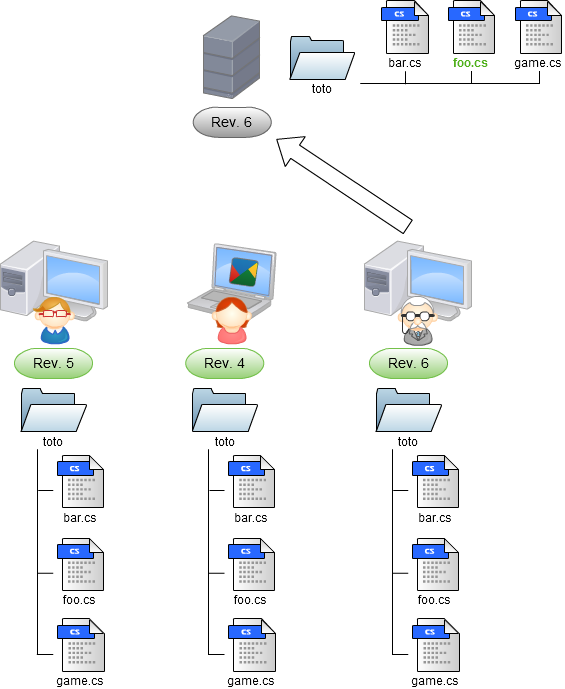
\includegraphics[scale=0.3]{images/6-Commit2.png}
  \end{center}
\end{frame}

\begin{frame}
  \begin{center}
    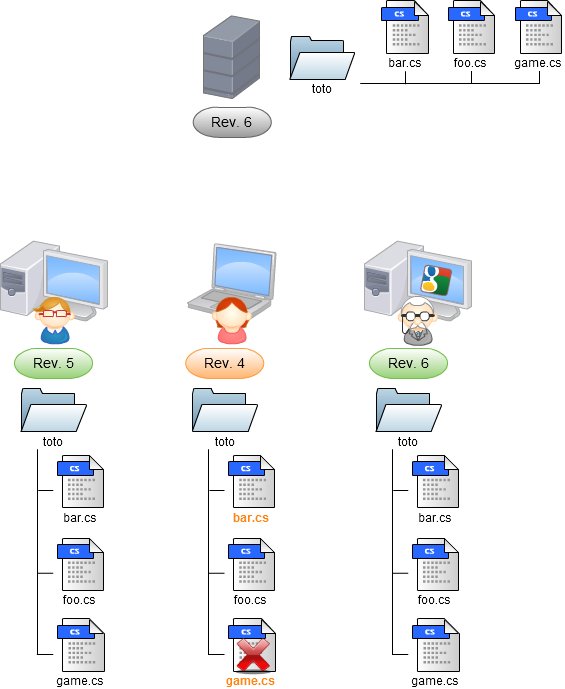
\includegraphics[scale=0.3]{images/7-Work.png}
  \end{center}
\end{frame}

\begin{frame}
  \begin{center}
    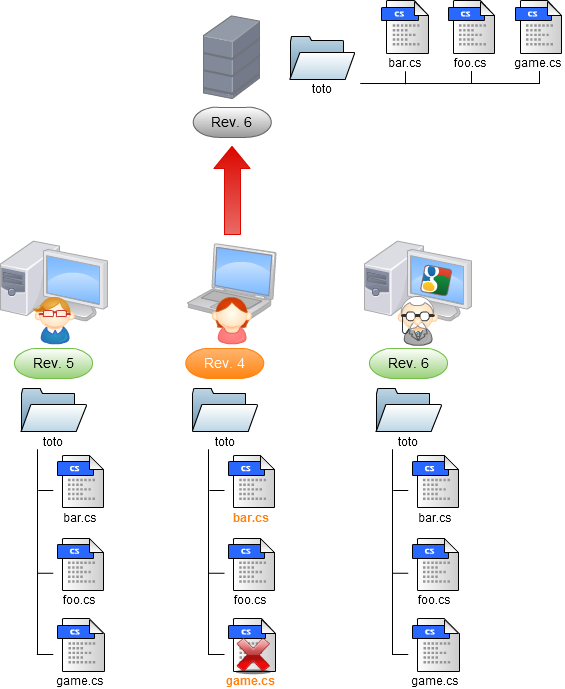
\includegraphics[scale=0.3]{images/8-Commit3.png}
  \end{center}
\end{frame}

\begin{frame}
  \begin{center}
    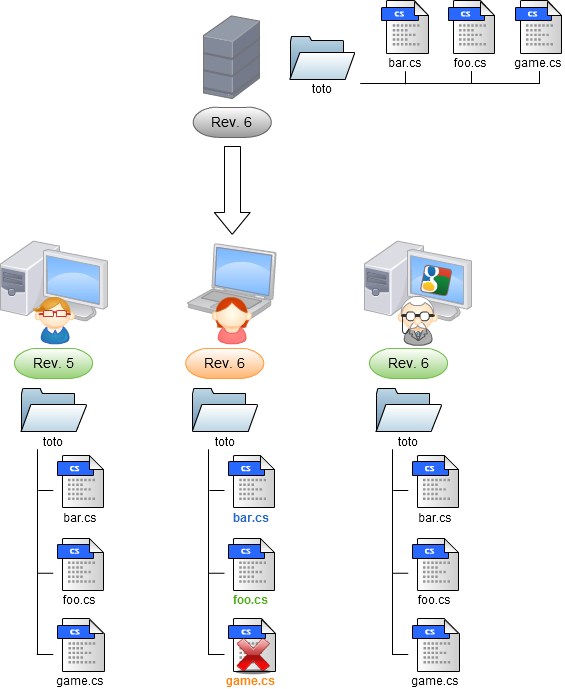
\includegraphics[scale=0.3]{images/9-Update_merge.png}
  \end{center}
\end{frame}

\begin{frame}
  \begin{center}
    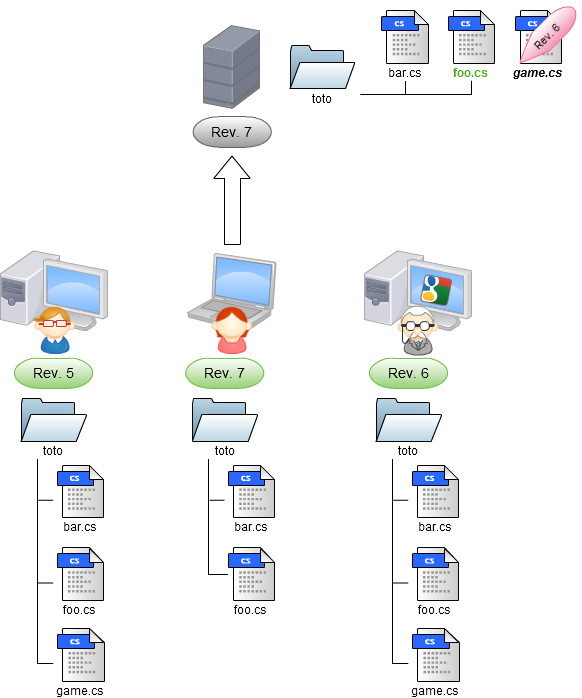
\includegraphics[scale=0.3]{images/10-Commit4.png}
  \end{center}
\end{frame}

\begin{frame}
  \begin{center}
    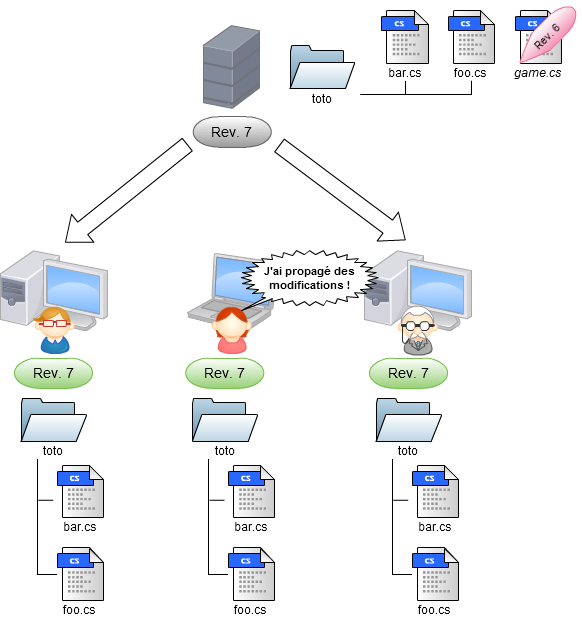
\includegraphics[scale=0.3]{images/11-Update.png}
  \end{center}
\end{frame}

\begin{frame}
  \begin{center}
    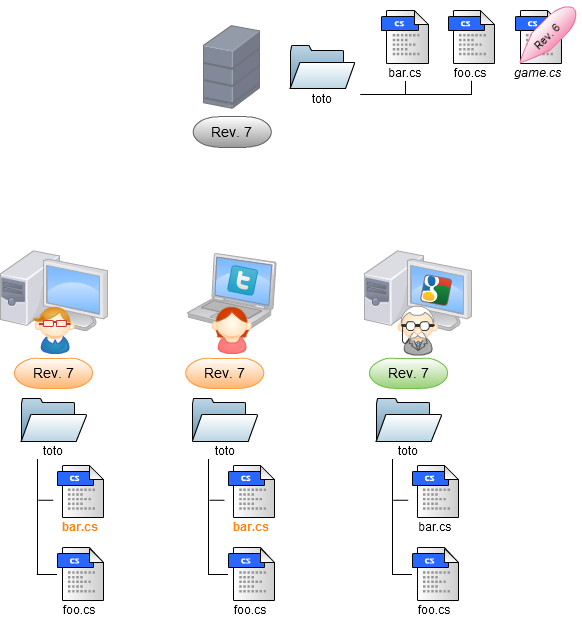
\includegraphics[scale=0.3]{images/12-Work.png}
  \end{center}
\end{frame}

\begin{frame}
  \begin{center}
    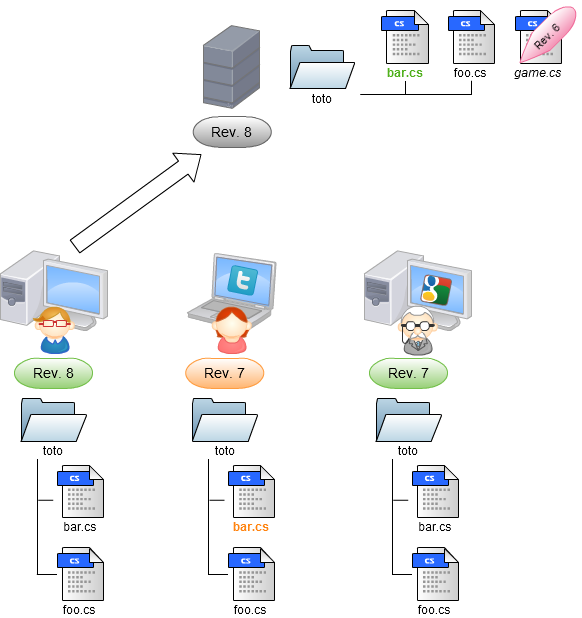
\includegraphics[scale=0.3]{images/13-Commit4.png}
  \end{center}
\end{frame}

\begin{frame}
  \begin{center}
    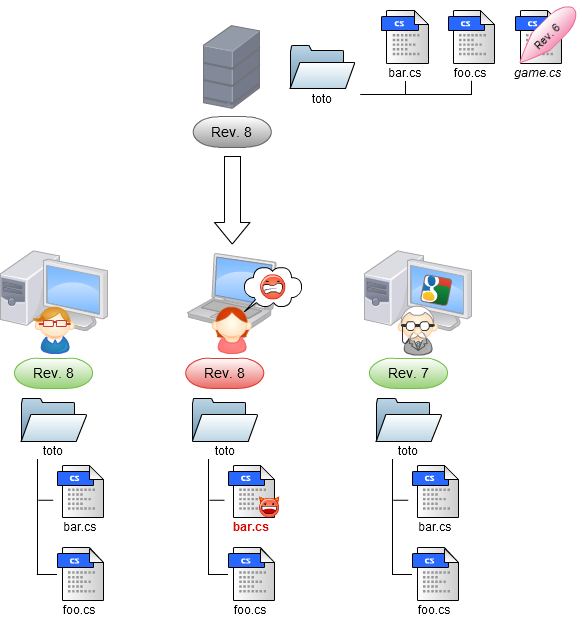
\includegraphics[scale=0.3]{images/14-Conflict.png}
  \end{center}
\end{frame}

\begin{frame}
  \begin{center}
    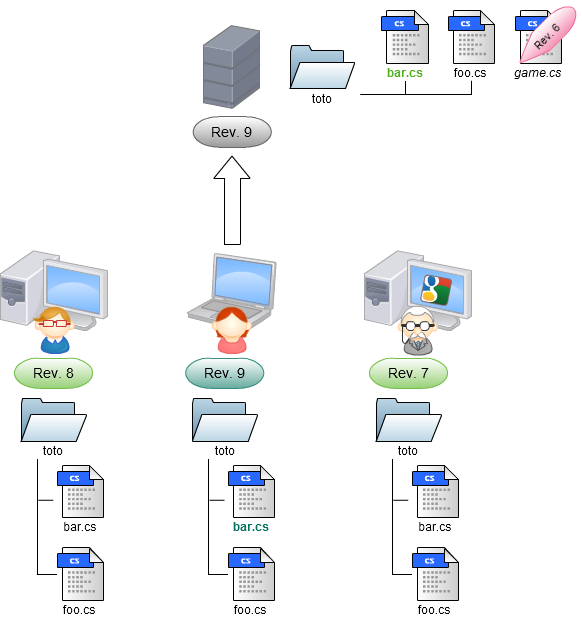
\includegraphics[scale=0.3]{images/15-Resolved.png}
  \end{center}
\end{frame}

\begin{frame}
  \begin{center}
    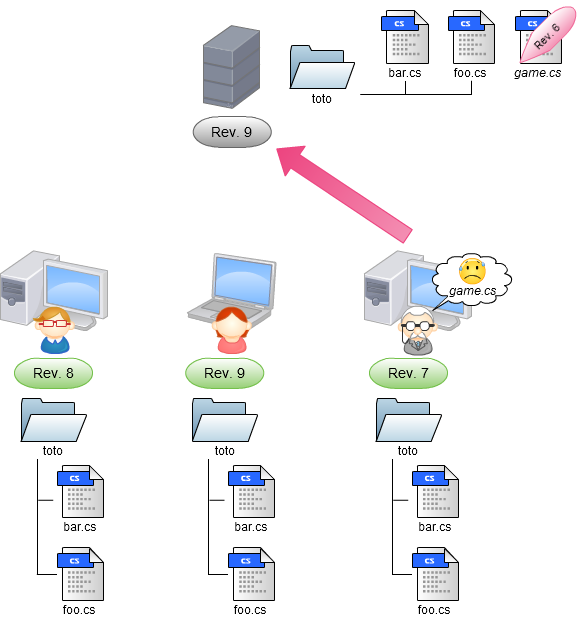
\includegraphics[scale=0.3]{images/16-Back1.png}
  \end{center}
\end{frame}


\subsection{Commandes usuelles}

\begin{frame}{Subversion survival package}
  \begin{block}{Checkout -- co}
    Récupération du contenu d'un dépôt (désigné par une URL) à une version donnée.
  \end{block}
  \begin{block}{Update -- up}
    Mise à jour du contenu d'un dossier/fichier sous versionnement par rapport à la référence.
  \end{block}
  \begin{block}{Commit -- ci}
    Enregistrement des modifications effectuées sur le serveur.
  \end{block}
  \begin{block}{Add}
    Activer le versionnement sur un dossier/fichier.
  \end{block}
\end{frame}

\subsection{Environnement de travail}
\begin{frame}
  \begin{center}
    
\includegraphics[scale=0.35]{images/logo_tortoise}
  \end{center}
  \begin{alertblock}{TortoiseSVN}
    \begin{itemize}
    \item S'intégre parfaitement à Windows,
    \item Ajout d'action sur les fichiers et dossiers (clic droit),
      \item Modification visuelle pour les dossiers et fichiers sous versionnement.
      \end{itemize}
    \end{alertblock}
\end{frame}

\begin{frame}
  \begin{figure}
    \begin{center}
      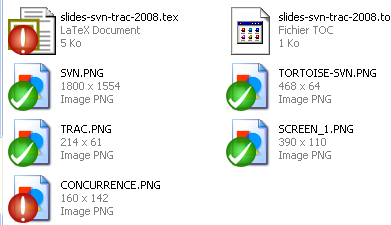
\includegraphics[scale=0.7]{images/dirView}
    \end{center}
  \end{figure}
\end{frame}
\begin{frame}
  \begin{figure}
    \begin{center}
      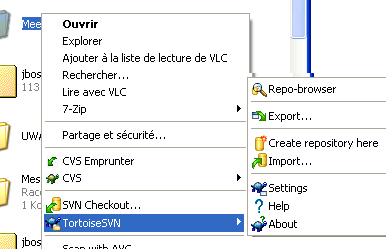
\includegraphics[scale=0.7]{images/actions}
    \end{center}
  \end{figure}
\end{frame}

\subsection{Bonnes pratiques}
\begin{frame}
  \begin{alertblock}{Update}
    Effectuer des updates régulièrement.
  \end{alertblock}
  \begin{alertblock}{Commit}
    Commiter \textbf{régulièrement} du code qui \textbf{compile}.
  \end{alertblock}
  \begin{alertblock}{Add}
    Ne pas mettre sous versionnement~:
    \begin{itemize}
    \item Les fichiers compilés par votre code (.exe, .o, .out, \ldots),
    \item Les fichiers propres à votre environnement de travail,
    \item Les fichiers systèmes (Thumbs.db, \ldots),
    \item Des fichiers inutiles (SVN n'est pas un système de partage de fichiers).
    \end{itemize}
  \end{alertblock}
\end{frame}

\subsection{Où trouver un dépôt~?}
\begin{frame}
  \begin{exampleblock}{Les dépôts gratuits}
    \begin{itemize}
    \item GoogleCode
    \item SourceForge
    \item Assembla
    \item svn.pc-show.com
    \end{itemize}
  \end{exampleblock}
\end{frame}
